\documentclass[aspectratio=43,display]{beamer}


\mode<presentation>
{
	\usetheme{Montpellier}	% or try Darmstadt, Madrid, Warsaw, ...
	\usecolortheme{rose}	% or try albatross, beaver, crane, dove...
	\usefonttheme{default}  % or try serif, structurebold, ...
	\setbeamertemplate{navigation symbols}{}
	\setbeamertemplate{caption}[numbered]
} 

\usepackage[english]{babel}
\usepackage[utf8x]{inputenc}
\usepackage{siunitx}
\usepackage{enumerate}
\usepackage{hyperref}
\usepackage{eso-pic}
\hypersetup{
	bookmarksopen=false,
	pdfpagemode=UseNone,
	%pdfpagemode=FullScreen,   %% Enable to have Adobe Reader query for fullscreen mode
	pdfauthor={Yuelin Xin} %% Enter the apppropriate author in here
}

\newcommand\AtPagemyUpperLeft[1]{\AtPageLowerLeft{%
		\put(\LenToUnit{0.75\paperwidth},\LenToUnit{0.9075\paperheight}){#1}}}
\AddToShipoutPictureFG{
	\AtPagemyUpperLeft{{
\includegraphics[width=3cm,keepaspectratio]{images/mf.png}}}
}%


\title[Scene Separation \& Data Selection]{Scene Separation \& Data Selection: Temporal Segmentation Algorithm for Real-time Video Stream Analysis}
%% Author with both abbreviation and affiliation
\author[YX, ZZ, YX]{Yuelin Xin\inst{1}\inst{2} \and Zihan Zhou\inst{1}\and Yuxuan Xia\inst{1}}
\institute[UL]{\inst{1}SWJTU-Leeds Joint School, CS\\Southwest Jiaotong University
	\and\inst{2}School of Computing\\University of Leeds}
\date[2022 STRL]{Spatio-Temporal Reasoning and Learning, 2022}


\begin{document}

	\begin{frame}
		\titlepage
	\end{frame}

	% Uncomment these lines for an automatically generated outline.
	\begin{frame}{Outline}
		\tableofcontents
	\end{frame}

	\section{Introduction}

		\begin{frame}{Introduction}

			\begin{itemize}
				\item The problem (Background \& What we want to achieve)
				\item Our motivation (Why not neural networks?)
			\end{itemize}

			\vskip 1cm

			\begin{block}{Remark}
				\textbf{Scene separation} is a problem in which we want to separate a video stream into different scenes.
				\textbf{A scene} is defined as a group of similar-looking frames that are temporally adjacent to each other.
			\end{block}

		\end{frame}


	\subsection{The problem}

		\begin{frame}{The problem}


			\begin{itemize}
				\item \textbf{Background}: real-time video stream interpretation, including video semantics / video accessibility / surveillance footage auto-interpretation, etc.
				\item \textbf{Difficulties}: algorithms do not see video as a continuous stream of images, but as discrete frames.
			\end{itemize}

			\vskip 0.3cm

			\begin{figure}
				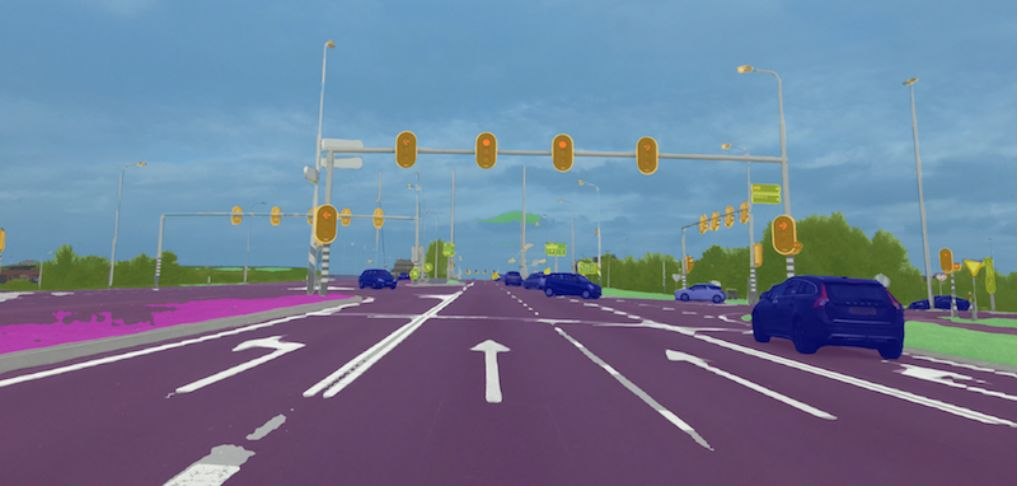
\includegraphics[width=5cm]{images/image-semantics.jpeg}
				\caption{\label{fig:your-figure}Video semantics.}
			\end{figure}

			% \begin{table}
			% \centering
			% \begin{tabular}{l|r}
			% Item & Quantity \\\hline
			% Widgets & 42 \\
			% Gadgets & 13
			% \end{tabular}
			% \caption{\label{tab:widgets}An example table.}
			% \end{table}

		\end{frame}


		\begin{frame}{The problem}

			\begin{itemize}
				\item \textbf{The traditional approach}: 3D CNNs (CNN models with the additional temporal dimension)
				\item \textbf{What's missing}: hard to control when the video is very long or it is of indefinite length (like live streaming).
			\end{itemize}

			\vskip 0.5cm

			\begin{block}{Example}
				It would be hard to pick up sudden moves in long videos because the longer the video, the worse the temporal resolution.
				(like a very tiny object in a very massive picture in 2D CNNs)
			\end{block}

		\end{frame}


	\subsection{Our motivation}

		\begin{frame}{Our motivation}

			Why not neural networks?

			\begin{itemize}
				\item \textbf{Neural networks are relatively slow}: the inference time of a lot of NNs makes them difficult to be used in real-time video analysis.
				\item And the 2SDS algorithm is fully capable of handling simple scene separation tasks.
			\end{itemize}

			% Let $X_1, X_2, \ldots, X_n$ be a sequence of independent and identically distributed random variables with $\text{E}[X_i] = \mu$ and $\text{Var}[X_i] = \sigma^2 < \infty$, and let
			% $$S_n = \frac{X_1 + X_2 + \cdots + X_n}{n}
			% 	= \frac{1}{n}\sum_{i}^{n} X_i$$
			% denote their mean. Then as $n$ approaches infinity, the random variables $\sqrt{n}(S_n - \mu)$ converge in distribution to a normal $\mathcal{N}(0, \sigma^2)$.

		\end{frame}


	\section{Method: 2SDS}

	\section{Our results}

	\section{Future improvements}

	\section{Conclusion}

\end{document}
